% ថ្នាក់ទី ១១ (វិទ្យាសាស្ត្រសង្គម) · ជំពូកទី ២ · មេរៀនទី ២ · សៀវភៅ ទំព័រ ៤៨–៦៨
\chapter{អនុគមន៍លោការីត}

\begin{objBox}[វត្ថុបំណង]
\begin{enumerate}[1]
  \item កំណត់អនុគមន៍ច្រាស
  \item សង់ក្រាបនៃអនុគមន៍លោការីត
  \item ដោះស្រាយសមីការនិងវិសមីការលោការីត
  \item អនុវត្តលើអនុគមន៍លោការីត ។
\end{enumerate}
\end{objBox}

\section{អនុគមន៍ច្រាស}
\subsection{និយមន័យអនុគមន៍ច្រាស}

\begin{example}[ឧទាហរណ៍ ១]
គេមានអនុគមន៍ $f$ និងអនុគមន៍ច្រាសកំណត់ដោយ $f^{-1}$ ។
\begin{center}
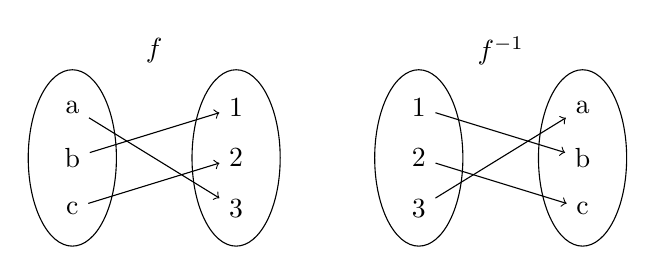
\begin{tikzpicture}[scale=0.8]
\draw (0,0) ellipse (0.7 and 1.4); \draw (2.6,0) ellipse (0.7 and 1.4);
\node at (1.3,1.7) {$f$};
\node (a) at (0,0.8) {a}; \node (b) at (0,0) {b}; \node (c) at (0,-0.8) {c};
\node (1) at (2.6,0.8) {1}; \node (2) at (2.6,0) {2}; \node (3) at (2.6,-0.8) {3};
\draw[->] (a) -- (3); \draw[->] (b) -- (1); \draw[->] (c) -- (2);
\begin{scope}[xshift=5.5cm]
\draw (0,0) ellipse (0.7 and 1.4); \draw (2.6,0) ellipse (0.7 and 1.4);
\node at (1.3,1.7) {$f^{-1}$};
\node (p) at (0,0.8) {1}; \node (q) at (0,0) {2}; \node (r) at (0,-0.8) {3};
\node (x) at (2.6,0.8) {a}; \node (y) at (2.6,0) {b}; \node (z) at (2.6,-0.8) {c};
\draw[->] (p) -- (y); \draw[->] (q) -- (z); \draw[->] (r) -- (x);
\end{scope}
\end{tikzpicture}
\end{center}
\end{example}

\begin{example}[ឧទាហរណ៍ ២]
គេមានអនុគមន៍ $f(x) = 2x + 5$ ។ គេបាន
\[
y = 2x + 5 \;\Rightarrow\; 2x = y - 5 \;\Rightarrow\; x = \frac{1}{2}y - \frac{5}{2} ។
\]
គេថាអនុគមន៍ $y = \dfrac{1}{2}x - \dfrac{5}{2}$ ហៅថាអនុគមន៍ច្រាសនៃ $f(x) = 2x + 5$ ដែលកំណត់សរសេរដោយ $f^{-1}(x) = \dfrac{1}{2}x - \dfrac{5}{2}$ ។
\end{example}

\begin{definition}[និយមន័យ]
អនុគមន៍ច្រាសនៃអនុគមន៍មួយ ជាអនុគមន៍ដែលបានមកពីការប្ដូរអថេរឯករាជ្យ $x$ ទៅជា $y$ ។
\end{definition}

\textbf{សង្កេត ៖} គេមានអនុគមន៍ពីរ $f(x) = 2x + 2$ និង $g(x) = \dfrac{x}{2} - 1$ ។
\begin{itemize}
  \item បើ $x = 1$ នោះ $f(1) = 4$ គេបានគូមានលំដាប់ $(1, 4)$ ហើយ $g(4) = 1$ ។
  \item បើ $x = 2$ នោះ $f(2) = 6$ គេបានគូមានលំដាប់ $(2, 6)$ ហើយ $g(6) = 2$ ។
  \item បើ $x = 3$ នោះ $f(3) = 8$ គេបានគូមានលំដាប់ $(3, 8)$ ហើយ $g(8) = 3$ ។
\end{itemize}
គូមានលំដាប់នៃអនុគមន៍ $f$ ច្រាសគ្នាទៅនឹងគូមានលំដាប់នៃអនុគមន៍ $g$ មានន័យថា ធាតុដើមតាម $f$ ប្រែក្លាយជារូបភាពតាម $g$ វិញ ហើយធាតុដើមតាម $g$ ប្រែក្លាយជារូបភាពតាម $f$ ។ ក្នុងករណីនេះ គេថា $g$ ជាអនុគមន៍ច្រាសនៃ $f$ ហើយ $f$ ក៏ជាអនុគមន៍ច្រាសនៃ $g$ ដែរ ។

\begin{formulaBox}[ជាទូទៅ]
បើ $(a, b)$ ផ្ទៀងផ្ទាត់ $y = f(x)$ ហើយ $(b, a)$ ផ្ទៀងផ្ទាត់ $y = f^{-1}(x)$ នោះ $f^{-1}$ ជាអនុគមន៍ច្រាសនៃអនុគមន៍ $f$ ។
\end{formulaBox}

\begin{example}[លំហាត់គំរូ]
កំណត់អនុគមន៍ច្រាសនៃ $f(x) = \dfrac{1}{x + 2}$ និង $g(x) = x^2$ ដែល $x \ge 0$ ។
\ans
\begin{itemize}
  \item $y = \dfrac{1}{x + 2}$ ឬ $y(x + 2) = 1$ គេបាន $x = \dfrac{1 - 2y}{y}$ ។ ដូច្នេះ $f^{-1}(x) = \dfrac{1 - 2x}{x}$ ។
  \item $y = x^2$ គេទាញបាន $x = \pm\sqrt{y}$ ដោយ $x \ge 0$ នោះ $x = \sqrt{y}$ ។ ដូច្នេះ $g^{-1}(x) = \sqrt{x}$ ។
\end{itemize}
\end{example}

\begin{pro}
កំណត់អនុគមន៍ច្រាសនៃ $f(x) = \dfrac{x - 1}{x}$ និង $g(x) = \sqrt{x} - 3$ ។
\ans
$f^{-1}(x) = \dfrac{1}{1 - x}$, \quad $g^{-1}(x) = (x + 3)^2$ ($x \ge -3$) ។
\end{pro}

\subsection{ក្រាបនៃអនុគមន៍ច្រាស}

\textbf{ឧទាហរណ៍ ៖} $f$ និង $f^{-1}$ ជាអនុគមន៍ច្រាសគ្នា ។ បើ $M(a, b) \in f$ នោះ $M'(b, a) \in f^{-1}$ ។ ដៅចំណុច $A(a, a)$ និង $B(b, b)$ គេបានការេ $AMBM'$ ។

$AB$ ជាបន្ទាត់មានសមីការ $y = x$ ព្រោះវាកាត់តាមចំណុចដែលមានអាប់ស៊ីសស្មើនឹងអរដោនេ ។ $M(a, b)$ និង $M'(b, a)$ ឆ្លុះគ្នាធៀបនឹងបន្ទាត់ $AB$ ។

ដូច្នេះក្រាបនៃ $f^{-1}$ ឆ្លុះនឹងក្រាបនៃ $f$ ធៀបនឹងបន្ទាត់ $y = x$ ។
\begin{center}
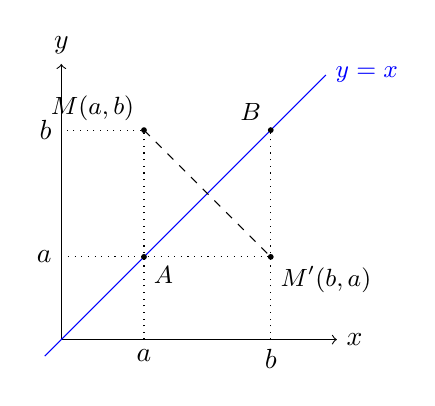
\begin{tikzpicture}[scale=0.7]
\draw[->] (0,0) -- (5,0) node[right] {$x$};
\draw[->] (0,0) -- (0,5) node[above] {$y$};
\draw[blue] (-0.3,-0.3) -- (4.8,4.8) node[right] {\small $y = x$};
\draw[dotted] (1.5,0) node[below] {$a$} -- (1.5,3.8) -- (0,3.8) node[left] {$b$};
\draw[dotted] (3.8,0) node[below] {$b$} -- (3.8,3.8);
\draw[dotted] (0,1.5) node[left] {$a$} -- (3.8,1.5);
\draw[dashed] (1.5,3.8) -- (3.8,1.5);
\fill (1.5,3.8) circle (1.5pt) node[above left] {\small $M(a,b)$};
\fill (3.8,1.5) circle (1.5pt) node[below right] {\small $M'(b,a)$};
\fill (1.5,1.5) circle (1.5pt) node[below right] {\small $A$};
\fill (3.8,3.8) circle (1.5pt) node[above left] {\small $B$};
\end{tikzpicture}
\end{center}

\begin{formulaBox}[ជាទូទៅ]
បើអនុគមន៍ពីរ $f(x)$ និង $g(x)$ ច្រាសគ្នា នោះក្រាបនៃអនុគមន៍ទាំងពីរឆ្លុះគ្នាធៀបនឹងបន្ទាត់ $y = x$ ។
\end{formulaBox}

\begin{example}[លំហាត់គំរូ ១]
គេឱ្យអនុគមន៍ $f(x) = \sqrt{x}$ ដែល $x \ge 0$ ។ ចូរកំណត់អនុគមន៍ច្រាសនៃ $f$ រួចសង់ក្រាបរបស់វា ។
\ans
$y = \sqrt{x}$ គេបាន $x = y^2$ ។ ដូច្នេះ $f^{-1}(x) = x^2$ ($x \ge 0$) ជាអនុគមន៍ច្រាសនៃ $f(x) = \sqrt{x}$ ។
\[
\begin{array}{|c|c||c|c|}\hline
x & f(x) = \sqrt{x} & x & f^{-1}(x) = x^2\\ \hline
0 & 0 & 0 & 0\\
1 & 1 & 1 & 1\\
4 & 2 & 2 & 4\\ \hline
\end{array}
\]
\begin{center}
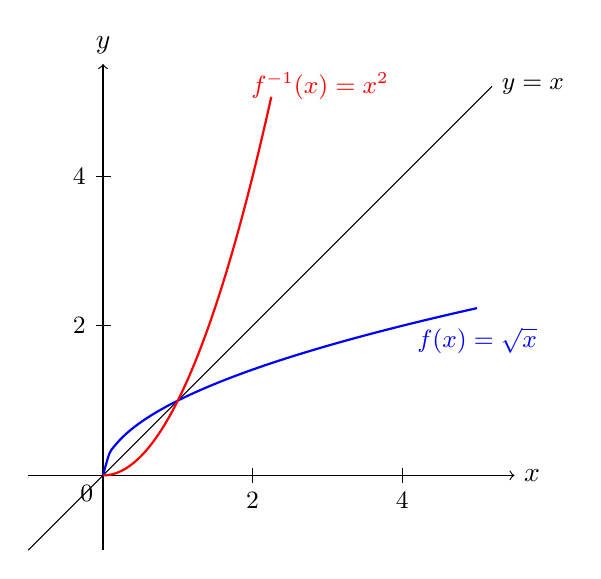
\begin{tikzpicture}[scale=0.95]
\draw[->] (-1,0) -- (5.5,0) node[right] {$x$};
\draw[->] (0,-1) -- (0,5.5) node[above] {$y$};
\draw (-1,-1) -- (5.2,5.2) node[right] {\small $y = x$};
\draw[thick,blue,domain=0:5,samples=60,smooth] plot (\x,{sqrt(\x)});
\draw[thick,red,domain=0:2.25,samples=60,smooth] plot (\x,{(\x)^2});
\node[blue] at (5,1.8) {\small $f(x) = \sqrt{x}$};
\node[red] at (2.9,5.2) {\small $f^{-1}(x) = x^2$};
\foreach \t in {2,4} {\draw (\t,0.1) -- (\t,-0.1) node[below] {\small $\t$}; \draw (0.1,\t) -- (-0.1,\t) node[left] {\small $\t$};}
\node[below left] at (0,0) {\small $0$};
\end{tikzpicture}
\end{center}
ក្រាបនៃអនុគមន៍ $f$ ឆ្លុះគ្នានឹង $f^{-1}$ ធៀបនឹងបន្ទាត់ $y = x$ ។
\end{example}

\begin{example}[លំហាត់គំរូ ២]
គេឱ្យអនុគមន៍ $g(x) = 2x - 1$ ។ ចូរកំណត់អនុគមន៍ច្រាស $g^{-1}$ រួចសង់ក្រាបរបស់វា ។
\ans
$y = 2x - 1$ គេបាន $x = \dfrac{1 + y}{2} = \dfrac{y}{2} + \dfrac{1}{2}$ ។ ដូច្នេះ $g^{-1}(x) = \dfrac{x}{2} + \dfrac{1}{2}$ ។
\[
\begin{array}{|c|c||c|c|}\hline
x & g(x) = 2x - 1 & x & g^{-1}(x) = \frac{x}{2} + \frac{1}{2}\\ \hline
0 & -1 & -1 & 0\\[2pt]
\frac{1}{2} & 0 & 0 & \frac{1}{2}\\[2pt] \hline
\end{array}
\]
\begin{center}
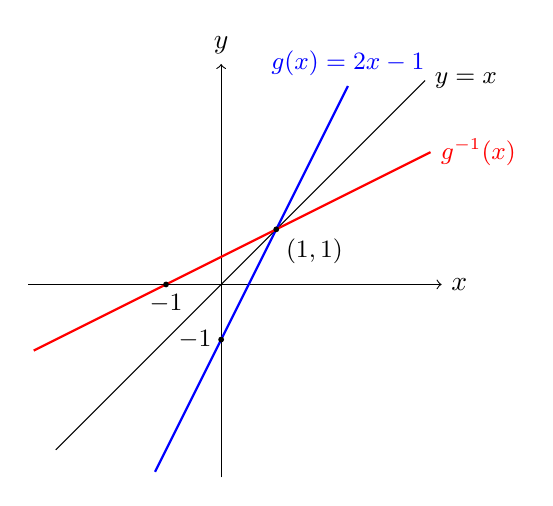
\begin{tikzpicture}[scale=0.7]
\draw[->] (-3.5,0) -- (4,0) node[right] {$x$};
\draw[->] (0,-3.5) -- (0,4) node[above] {$y$};
\draw (-3,-3) -- (3.7,3.7) node[right] {\small $y = x$};
\draw[thick,blue,domain=-1.2:2.3] plot (\x,{2*\x-1}) node[above] {\small $g(x) = 2x - 1$};
\draw[thick,red,domain=-3.4:3.8] plot (\x,{\x/2+0.5}) node[right] {\small $g^{-1}(x)$};
\fill (1,1) circle (1.5pt) node[below right] {\small $(1,1)$};
\fill (0,-1) circle (1.5pt) node[left] {\small $-1$};
\fill (-1,0) circle (1.5pt) node[below] {\small $-1$};
\end{tikzpicture}
\end{center}
ក្រាបនៃ $g$ និង $g^{-1}$ ឆ្លុះគ្នាធៀបនឹងបន្ទាត់ $y = x$ ហើយកាត់គ្នាត្រង់ $(1, 1)$ ។
\end{example}

\begin{pro}
គេឱ្យអនុគមន៍ $f(x) = -\dfrac{x}{2} + 1$ ។ កំណត់អនុគមន៍ច្រាស $f^{-1}(x)$ រួចសង់ក្រាបរបស់វា ។
\ans
$f^{-1}(x) = 2 - 2x$ ។ ក្រាបទាំងពីរជាបន្ទាត់ឆ្លុះគ្នាធៀបនឹង $y = x$ ហើយកាត់គ្នាត្រង់ $\left(\frac{2}{3}, \frac{2}{3}\right)$ ។
\end{pro}

\section{អនុគមន៍លោការីត}
\subsection{សញ្ញាណលោការីត}

\begin{example}[ឧទាហរណ៍]
ក. $(-2)^3 = -8$ \quad ខ. $1^3 = 1$ \quad គ. $0^3 = 0$
\begin{itemize}
  \item[ឃ.] $2^3 = 8$ ៖ $3$ ហៅថាលោការីតគោល $2$ នៃ $8$ ដែលកំណត់សរសេរ $3 = \log_2 8$ ។
  \item[ង.] $2^{-3} = \dfrac{1}{8}$ ៖ $-3$ ហៅថាលោការីតគោល $2$ នៃ $\dfrac{1}{8}$ ដែលកំណត់សរសេរ $-3 = \log_2\dfrac{1}{8}$ ។
\end{itemize}
\end{example}

\begin{definition}[និយមន័យ]
\textbf{លោការីត} គឺជាតម្លៃនិទស្សន្តនៃស្វ័យគុណ ដែលមានគោលជាចំនួនវិជ្ជមានខុសពី $1$ ។
\[
a^x = y \iff \log_a y = x, \qquad a > 0,\ a \ne 1,\ y > 0 ។
\]
\end{definition}

\subsection{អនុគមន៍លោការីត}
\textbf{ឧទាហរណ៍ ៖} គេមានអនុគមន៍អិចស្ប៉ូណង់ស្យែល $y = a^x$ នោះ $x = \log_a y$ ។ គេទាញបានអនុគមន៍ $y = \log_a x$ ជាអនុគមន៍ច្រាសនៃអនុគមន៍អិចស្ប៉ូណង់ស្យែល $y = a^x$ ។

\begin{definition}[និយមន័យ]
\textbf{អនុគមន៍លោការីត} គឺជាអនុគមន៍ច្រាសនៃអនុគមន៍អិចស្ប៉ូណង់ស្យែល ។ បើគេមាន $a^x = y$ នោះ $x = \log_a y$ ($y > 0$, $a > 0$, $a \ne 1$) ហើយ $f(x) = a^x$ មានអនុគមន៍ច្រាស $f^{-1}(x) = \log_a x$ ជាអនុគមន៍លោការីតគោល $a$ នៃ $x$ ។
\end{definition}
ករណី $a = 10$, $\log_{10} x$ ហៅថា \textbf{លោការីតទសភាគ} គេអាចសរសេរដោយងាយ $\log x$ ។

\begin{example}[លំហាត់គំរូ]
គណនា $\log_2 64$, $\log_3 243$, $\log_2\dfrac{1}{16}$, $\log_2 1$ ។
\ans
គេប្រើ $a^x = y \iff x = \log_a y$ ។
\begin{itemize}
  \item តាង $\log_2 64 = x$ សមមូល $2^x = 64 = 2^6$ គេបាន $x = 6$ ។ ដូច្នេះ $\log_2 64 = 6$ ។
  \item តាង $\log_3 243 = x$ សមមូល $3^x = 243 = 3^5$ គេបាន $x = 5$ ។ ដូច្នេះ $\log_3 243 = 5$ ។
  \item តាង $\log_2\frac{1}{16} = x$ សមមូល $2^x = \frac{1}{16} = 2^{-4}$ គេបាន $x = -4$ ។ ដូច្នេះ $\log_2\frac{1}{16} = -4$ ។
  \item តាង $\log_2 1 = x$ សមមូល $2^x = 1 = 2^0$ គេបាន $x = 0$ ។ ដូច្នេះ $\log_2 1 = 0$ ។
\end{itemize}
\end{example}

\begin{pro}
គណនា ៖ \quad ក. $\log_5 125$ \quad ខ. $\log_4\dfrac{1}{4}$ \quad គ. $\log_{\frac{1}{2}} 25$ \quad ឃ. $\log_2 2$ ។
\ans
ក. $3$ \quad ខ. $-1$ \quad គ. $\log_{\frac{1}{2}} 25 = -\log_2 25 = -2\log_2 5 \approx -4.64$ \quad ឃ. $1$ ។
\end{pro}

\subsection{លក្ខណៈនៃលោការីត}
ដោយ $a^1 = a$ នោះ $\log_a a = 1$ ហើយ $a^0 = 1$ នោះ $\log_a 1 = 0$ ។

\begin{theorem}[លក្ខណៈលោការីត]
ចំពោះគ្រប់ចំនួនវិជ្ជមាន $x$, $y$ និង $a$ ដែល $a \ne 1$ គេបាន ៖
\begin{enumerate}[1]
  \item $\log_a(xy) = \log_a x + \log_a y$
  \item $\log_a x^n = n\log_a x$
  \item $\log_a a = 1$
  \item $\log_a a^x = x$
  \item $\log_a\left(\dfrac{x}{y}\right) = \log_a x - \log_a y$
  \item $\log_a x = \dfrac{1}{\log_x a}$ \quad ($x \ne 1$)
  \item $\log_a 1 = 0$
  \item $a^{\log_a x} = x$ ។
\end{enumerate}
\end{theorem}

\textbf{សម្រាយបញ្ជាក់ ៖} តាង $m = \log_a x$ នោះ $a^m = x$ និង $n = \log_a y$ នោះ $a^n = y$ ។
\begin{enumerate}[1]
  \item $x\times y = a^m\times a^n = a^{m+n}$ នោះ $\log_a(xy) = m + n$ ។ ដូច្នេះ $\log_a(xy) = \log_a x + \log_a y$ ។
  \item $\dfrac{x}{y} = \dfrac{a^m}{a^n} = a^{m-n}$ នោះ $m - n = \log_a\dfrac{x}{y}$ ។ ដូច្នេះ $\log_a\dfrac{x}{y} = \log_a x - \log_a y$ ។
  \item តាមលក្ខណៈវិធីគុណ ៖
  \[
  \begin{aligned}
  \log_a x^n &= \log_a\underbrace{(x\times x\times\cdots\times x)}_{n \text{ កត្តា}}\\
  &= \underbrace{\log_a x + \log_a x + \cdots + \log_a x}_{n \text{ តួ}} = n\log_a x ។
  \end{aligned}
  \]
  \item តាង $m = \log_a x$ នោះ $x = a^m$ ហើយ $n = \log_x a$ នោះ $a = x^n$ ។ គេបាន $x = a^m = (x^n)^m = x^{mn}$ នាំឱ្យ $mn = 1$ ។ ដូច្នេះ $(\log_a x)(\log_x a) = 1$ ឬ $\log_a x = \dfrac{1}{\log_x a}$ ។
\end{enumerate}

\begin{example}[លំហាត់គំរូ ១]
គណនា ៖ \quad ក. $\log_2(4\times 16)$ \quad ខ. $\log_2 45 + \log_2 2$ \quad គ. $3\log_7 4 - 2\log_7 8$ \quad ឃ. $\log_2 4 + \log_4 2$ ។
\ans
ក. $\log_2(4\times 16) = \log_2 4 + \log_2 16 = \log_2 2^2 + \log_2 2^4 = 2 + 4 = 6$ ។\\
ខ. $\log_2 45 + \log_2 2 = \log_2(45\times 2) = \log_2 90$ ។\\
គ. $3\log_7 4 - 2\log_7 8 = \log_7 4^3 - \log_7 8^2 = \log_7\dfrac{64}{64} = \log_7 1 = 0$ ។\\
ឃ. $\log_2 4 + \log_4 2 = \log_2 4 + \dfrac{1}{\log_2 4} = 2 + \dfrac{1}{2} = \dfrac{5}{2}$ ។
\end{example}

\begin{formulaBox}[រូបមន្តប្ដូរគោល]
បើ $a \ne 1$, $a > 0$, $b > 0$, $b \ne 1$ និង $x$ ជាចំនួនវិជ្ជមាន នោះ
\[
\log_a x = \frac{\log_b x}{\log_b a} ។
\]
\end{formulaBox}
\textbf{សម្រាយបញ្ជាក់ ៖} តាង $y = \log_a x$ នោះ $a^y = x$ ។ គេបាន $\log_b a^y = \log_b x$ ឬ $y\log_b a = \log_b x$ ។ ដូច្នេះ $\log_a x = \dfrac{\log_b x}{\log_b a}$ ។

\begin{example}[លំហាត់គំរូ ២]
គណនា $\log_5 89$ និង $\log_{\sqrt{2}}\sqrt{5}$ ។
\ans
\[
\log_5 89 = \frac{\log 89}{\log 5} \approx \frac{1.94939}{0.69897} \approx 2.7889
\]
\[
\log_{\sqrt{2}}\sqrt{5} = \frac{\log\sqrt{5}}{\log\sqrt{2}} = \frac{\frac{1}{2}\log 5}{\frac{1}{2}\log 2} \approx \frac{0.69897}{0.30103} \approx 2.3219 ។
\]
\end{example}

\begin{pro}
\textbf{(ប្រតិបត្តិ ១)} ពន្លាតជាផលបូកឬផលគុណនៃលោការីត ៖
\begin{tasks}(4)
  \task $\log_a MN$
  \task $\log_3(8\times 3)$
  \task $\log_2(16\times 3)$
  \task $\log_a(xyz)$
  \task $\log_4 5^7$
  \task $\log_a\sqrt[3]{5}$
  \task $\log_2\sqrt[4]{3}$
  \task $\log_2\sqrt[3]{a}$
\end{tasks}
\ans
ក. $\log_a M + \log_a N$ \quad ខ. $3\log_3 2 + 1$ \quad គ. $4 + \log_2 3$ \quad ឃ. $\log_a x + \log_a y + \log_a z$ \quad ង. $7\log_4 5$ \quad ច. $\frac{1}{3}\log_a 5$ \quad ឆ. $\frac{1}{4}\log_2 3$ \quad ជ. $\frac{1}{3}\log_2 a$ ។
\end{pro}

\begin{pro}
\textbf{(ប្រតិបត្តិ ២)} គណនា ៖
\begin{tasks}(3)
  \task $\log_{0.5}\sqrt[3]{4}$
  \task $\log_{0.2} 25^{\frac{2}{3}}$
  \task $\log_{\sqrt{5}}(0.5)^{\frac{4}{3}}$
  \task $\log_{\sqrt[3]{7}}\log_2 2^{\sqrt{3}}$
  \task $\log_a x + \log_a y - \log_a z$
  \task $\log_a\sqrt{x} - \frac{1}{2}\log_a y$
\end{tasks}
\ans
ក. $-\dfrac{2}{3}$ \quad ខ. $-\dfrac{4}{3}$ \quad គ. $-\dfrac{8}{3}\log_5 2 \approx -1.15$ \quad ឃ. $\log_{\sqrt[3]{7}}\sqrt{3} = \dfrac{3}{2}\log_7 3 \approx 0.85$ \quad ង. $\log_a\dfrac{xy}{z}$ \quad ច. $\log_a\sqrt{\dfrac{x}{y}}$ ។
\end{pro}

\subsection{ក្រាបនៃអនុគមន៍លោការីត}

\begin{example}[ឧទាហរណ៍ ១]
គណនាតម្លៃលេខនិងសង់ក្រាបនៃអនុគមន៍ $y = \log_2 x$ ។
\ans
\[
\begin{array}{|c|ccccc|}\hline
x & -2 & -1 & 0 & 1 & 2\\ \hline
y = 2^x & 0.25 & 0.5 & 1 & 2 & 4\\ \hline\hline
x & 0.25 & 0.5 & 1 & 2 & 4\\ \hline
y = \log_2 x & -2 & -1 & 0 & 1 & 2\\ \hline
\end{array}
\]
\begin{center}
\begin{tikzpicture}[scale=0.8]
\draw[->] (-4.5,0) -- (6,0) node[right] {$x$};
\draw[->] (0,-4) -- (0,6) node[above] {$y$};
\draw (-3,-3) -- (5.5,5.5) node[right] {\small $y = x$};
\draw[thick,blue,domain=-4.5:2.5,samples=60,smooth] plot (\x,{2^(\x)}) node[above] {\small $y = 2^x$};
\draw[thick,red,domain=0.06:5.8,samples=80,smooth] plot (\x,{ln(\x)/ln(2)}) node[right] {\small $y = \log_2 x$};
\foreach \t in {1,4} {\draw (\t,0.1) -- (\t,-0.1) node[below] {\small $\t$}; \draw (0.1,\t) -- (-0.1,\t) node[left] {\small $\t$};}
\node[below left] at (0,0) {\small $0$};
\end{tikzpicture}
\end{center}
តម្លៃ $x$ កើន គេបានតម្លៃត្រូវគ្នានៃ $y = \log_2 x$ កើន ហើយក្រាបនៃ $y = \log_2 x$ កាត់អ័ក្ស $(Ox)$ ត្រង់ចំណុច $(1, 0)$ ។ អនុគមន៍ $y = \log_2 x$ និង $y = 2^x$ ជាអនុគមន៍ច្រាសគ្នា ដូច្នេះក្រាបរបស់វាឆ្លុះគ្នាធៀបនឹងបន្ទាត់ $y = x$ ។
\end{example}

\begin{example}[ឧទាហរណ៍ ២]
គណនាតម្លៃលេខនិងសង់ក្រាបនៃអនុគមន៍ $y = \log_{\frac{1}{2}} x$ ។
\ans
\[
\begin{array}{|c|ccccc|}\hline
x & -2 & -1 & 0 & 1 & 2\\ \hline
y = \left(\frac{1}{2}\right)^x & 4 & 2 & 1 & 0.5 & 0.25\\ \hline\hline
x & 0.25 & 0.5 & 1 & 2 & 4\\ \hline
y = \log_{\frac{1}{2}} x & 2 & 1 & 0 & -1 & -2\\ \hline
\end{array}
\]
\begin{center}
\begin{tikzpicture}[scale=0.8]
\draw[->] (-4.5,0) -- (6.5,0) node[right] {$x$};
\draw[->] (0,-4) -- (0,6) node[above] {$y$};
\draw (-3,-3) -- (5.5,5.5) node[right] {\small $y = x$};
\draw[thick,blue,domain=-2.5:6.3,samples=60,smooth] plot (\x,{0.5^(\x)});
\node[blue] at (-3.2,5.2) {\small $y = \left(\frac{1}{2}\right)^x$};
\draw[thick,red,domain=0.03:6.3,samples=80,smooth] plot (\x,{-ln(\x)/ln(2)});
\node[red] at (5.2,-3.3) {\small $y = \log_{\frac{1}{2}} x$};
\foreach \t in {1,4} {\draw (\t,0.1) -- (\t,-0.1) node[below] {\small $\t$}; \draw (0.1,\t) -- (-0.1,\t) node[left] {\small $\t$};}
\node[below left] at (0,0) {\small $0$};
\end{tikzpicture}
\end{center}
តម្លៃ $x$ កើន គេបានតម្លៃត្រូវគ្នានៃ $y = \log_{\frac{1}{2}} x$ ចុះ ហើយក្រាបកាត់អ័ក្ស $(Ox)$ ត្រង់ចំណុច $(1, 0)$ ។ ក្រាបនៃ $y = \log_{\frac{1}{2}} x$ និង $y = \left(\frac{1}{2}\right)^x$ ឆ្លុះគ្នាធៀបនឹងបន្ទាត់ $y = x$ ។
\end{example}

\begin{formulaBox}[ជាទូទៅ]
អនុគមន៍ $y = a^x$ និង $y = \log_a x$ ដែល $a > 0$, $a \ne 1$ មានក្រាបឆ្លុះគ្នាធៀបនឹងបន្ទាត់ $y = x$ ៖
\begin{center}
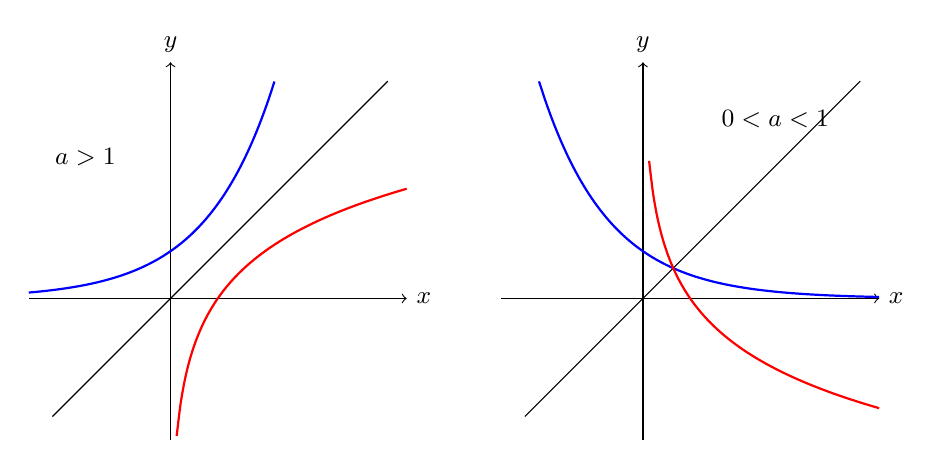
\begin{tikzpicture}[scale=0.6]
\draw[->] (-3,0) -- (5,0) node[right] {\small $x$};
\draw[->] (0,-3) -- (0,5) node[above] {\small $y$};
\draw (-2.5,-2.5) -- (4.6,4.6);
\draw[thick,blue,domain=-3:2.2,samples=50,smooth] plot (\x,{2^(\x)});
\draw[thick,red,domain=0.13:5,samples=60,smooth] plot (\x,{ln(\x)/ln(2)});
\node at (-1.8,3) {\small $a > 1$};
\begin{scope}[xshift=10cm]
\draw[->] (-3,0) -- (5,0) node[right] {\small $x$};
\draw[->] (0,-3) -- (0,5) node[above] {\small $y$};
\draw (-2.5,-2.5) -- (4.6,4.6);
\draw[thick,blue,domain=-2.2:5,samples=50,smooth] plot (\x,{0.5^(\x)});
\draw[thick,red,domain=0.13:5,samples=60,smooth] plot (\x,{-ln(\x)/ln(2)});
\node at (2.8,3.8) {\small $0 < a < 1$};
\end{scope}
\end{tikzpicture}
\end{center}
(ខ្សែពណ៌ខៀវ ៖ $y = a^x$, ខ្សែពណ៌ក្រហម ៖ $y = \log_a x$)
\end{formulaBox}

យើងសង្កេតឃើញថា អនុគមន៍ $y = \log_a x$ មានក្រាប ៖
\begin{itemize}
  \item បើ $a > 1$ ក្រាបកើនពីឆ្វេងទៅស្ដាំ គេថា $y = \log_a x$ ជាអនុគមន៍កើន ៖ ករណី $0 < x < 1$ តម្លៃ $\log_a x < 0$ ហើយករណី $x > 1$ តម្លៃ $\log_a x > 0$ ។
  \item បើ $0 < a < 1$ ក្រាបចុះពីឆ្វេងទៅស្ដាំ គេថា $y = \log_a x$ ជាអនុគមន៍ចុះ ៖ ករណី $0 < x < 1$ តម្លៃ $\log_a x > 0$ ហើយករណី $x > 1$ តម្លៃ $\log_a x < 0$ ។
  \item អនុគមន៍ $y = \log_a x$ មានក្រាបកាត់តាមចំណុច $(1, 0)$ ជានិច្ច ។
  \item អនុគមន៍ $y = \log_a x$ មានន័យចំពោះ $x > 0$ ជានិច្ច ។
  \item អនុគមន៍ $y = \log_a x$ និង $y = a^x$ មានក្រាបឆ្លុះគ្នាធៀបនឹងបន្ទាត់ $y = x$ ។
\end{itemize}

\begin{example}[លំហាត់គំរូ]
សង់ក្រាបនៃអនុគមន៍ ៖ \quad ក. $y = \log_3 x$ \quad ខ. $y = \log_{\frac{1}{3}} x$ ។
\ans
តារាងតម្លៃត្រូវគ្នានៃ $x$ និង $y$ ៖
\[
\begin{array}{|c|ccccc|}\hline
x & \frac{1}{9} & \frac{1}{3} & 1 & 3 & 9\\[2pt] \hline
y = \log_3 x & -2 & -1 & 0 & 1 & 2\\ \hline
y = \log_{\frac{1}{3}} x & 2 & 1 & 0 & -1 & -2\\ \hline
\end{array}
\]
\begin{center}
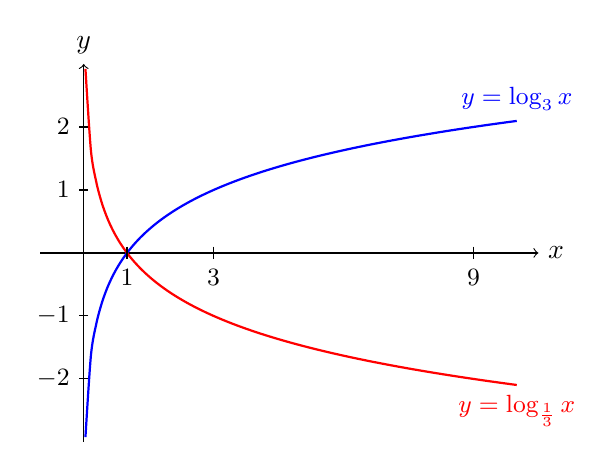
\begin{tikzpicture}[x=0.55cm,y=0.8cm]
\draw[->] (-1,0) -- (10.5,0) node[right] {$x$};
\draw[->] (0,-3) -- (0,3) node[above] {$y$};
\draw[thick,blue,domain=0.04:10,samples=80,smooth] plot (\x,{ln(\x)/ln(3)}) node[above] {\small $y = \log_3 x$};
\draw[thick,red,domain=0.04:10,samples=80,smooth] plot (\x,{-ln(\x)/ln(3)}) node[below] {\small $y = \log_{\frac{1}{3}} x$};
\foreach \t in {1,3,9} \draw (\t,0.1) -- (\t,-0.1) node[below] {\small $\t$};
\foreach \t in {-2,-1,1,2} \draw (0.1,\t) -- (-0.1,\t) node[left] {\small $\t$};
\end{tikzpicture}
\end{center}
ក្រាបនៃ $y = \log_3 x$ ជាអនុគមន៍កើន ព្រោះគោលធំជាង $1$ ហើយក្រាបនៃ $y = \log_{\frac{1}{3}} x$ ជាអនុគមន៍ចុះ ព្រោះ $0 < \frac{1}{3} < 1$ ។
\end{example}

\begin{pro}
សង់ក្រាបនៃអនុគមន៍ ៖ \quad ក. $y = \log_7 x$ \quad ខ. $y = \log_{\frac{1}{7}} x$ ។
\ans
ក. ក្រាបកើន កាត់តាម $\left(\frac{1}{7}, -1\right)$, $(1, 0)$, $(7, 1)$ \quad ខ. ក្រាបចុះ កាត់តាម $\left(\frac{1}{7}, 1\right)$, $(1, 0)$, $(7, -1)$ ។ ក្រាបទាំងពីរឆ្លុះគ្នាធៀបនឹងអ័ក្ស $(Ox)$ ។
\end{pro}

\section{សមីការនិងវិសមីការលោការីត}
\subsection{សមីការលោការីត}
បើ $a > 0$, $a \ne 1$ នោះសមីការ $\log_a x = \log_a y$ គេបាន $x = y$ ។

\begin{example}[ឧទាហរណ៍ ១]
ដោះស្រាយសមីការ $\log_3(5x + 7) = 2$ ។
\ans
សមីការមានន័យកាលណា $5x + 7 > 0$ ឬ $x > -\dfrac{7}{5}$ ។
\[
\log_3(5x + 7) = 2 \iff 5x + 7 = 3^2 \quad (\text{តាមនិយមន័យលោការីត})
\]
$5x + 7 = 9$ នាំឱ្យ $x = \dfrac{2}{5}$ ។ ដូច្នេះសមីការមានឫស $x = \dfrac{2}{5}$ ។
\end{example}

\begin{example}[ឧទាហរណ៍ ២]
ដោះស្រាយសមីការ $\log x + \log(x + 3) = 1$ និងផ្ទៀងផ្ទាត់ ។
\ans
សមីការមានន័យលុះត្រាតែ $x > 0$ និង $x + 3 > 0$ នាំឱ្យ $x > 0$ ។
\[
\begin{aligned}
\log[x(x + 3)] &= 1 && \text{តាមលក្ខណៈលោការីតនៃផលគុណ}\\
x(x + 3) &= 10^1 && \text{សរសេរជារាងអិចស្ប៉ូណង់ស្យែល}\\
x^2 + 3x - 10 &= 0\\
(x + 5)(x - 2) &= 0 && \Rightarrow x = -5,\ x = 2
\end{aligned}
\]
\textbf{ផ្ទៀងផ្ទាត់ ៖} $x = -5$ មិនយក ព្រោះមិនផ្ទៀងផ្ទាត់លក្ខខណ្ឌ $x \in (0, +\infty)$ ។ $x = 2$ ផ្ទៀងផ្ទាត់លក្ខខណ្ឌ ។ ដូច្នេះ សមីការមានឫស $x = 2$ ។
\end{example}

\begin{example}[លំហាត់គំរូ]
ដោះស្រាយសមីការ ៖ \quad ក. $\log_6 x + \log_6(x - 5) = 2$ \quad ខ. $3\log_5 x - \log_5 4 = \log_5 16$ \quad គ. $\log_4 x + \log_4(x - 6) = 2$ ។
\ans
ក. សមីការមានន័យកាលណា $x > 0$ និង $x - 5 > 0$ ឬ $x > 5$ ។
\[
\begin{gathered}
\log_6 x(x - 5) = 2 = \log_6 6^2 \;\Rightarrow\; x^2 - 5x = 36\\
x^2 - 5x - 36 = 0 \;\Rightarrow\; (x + 4)(x - 9) = 0 \;\Rightarrow\; x = -4,\ x = 9
\end{gathered}
\]
$x = -4$ មិនយក ព្រោះមិនផ្ទៀងផ្ទាត់លក្ខខណ្ឌ ។ ដូច្នេះ សមីការមានឫស $x = 9$ ។

ខ. សមីការមានន័យកាលណា $x > 0$ ។ ដោយ $3\log_5 x = \log_5 x^3$ ៖
\[
\log_5\frac{x^3}{4} = \log_5 16 \;\Rightarrow\; x^3 = 64 \;\Rightarrow\; x = 4 ។
\]
ដូច្នេះ សមីការមានឫស $x = 4$ ។

គ. សមីការមានន័យកាលណា $x > 6$ ។
\[
\begin{gathered}
\log_4 x(x - 6) = 2 \;\Rightarrow\; x^2 - 6x = 4^2\\
x^2 - 6x - 16 = 0 \;\Rightarrow\; (x - 8)(x + 2) = 0 \;\Rightarrow\; x = 8,\ x = -2
\end{gathered}
\]
ដោយ $x = -2$ មិនបំពេញលក្ខខណ្ឌសមីការ ។ ដូច្នេះសមីការមានឫស $x = 8$ ។
\end{example}

\begin{pro}
ដោះស្រាយនិងផ្ទៀងផ្ទាត់សមីការខាងក្រោម ៖
\begin{tasks}(2)
  \task $\log_6\dfrac{1}{36} = -2x$
  \task $\log_x 9 = 2$
  \task $\log_3 5 + \log_3 x = \log_3 10$
  \task $\log_8(x^2 + x) = \log_8 12$
\end{tasks}
\ans
ក. $x = 1$ \quad ខ. $x = 3$ \quad គ. $x = 2$ \quad ឃ. $x = 3$ ឬ $x = -4$ ។
\end{pro}

\subsection{វិសមីការលោការីត}
តាមក្រាបនៃអនុគមន៍លោការីត $y = \log_a x$ គេសង្កេតឃើញថា ៖
\begin{itemize}
  \item បើ $a > 1$ នោះក្រាបនៃ $y = \log_a x$ កើនពីឆ្វេងទៅស្ដាំ មានន័យថា កាលណាតម្លៃ $x$ កើន តម្លៃនៃអនុគមន៍កើន ។ ដូច្នេះ បើ $\log_a x_1 < \log_a x_2$ គេបាន $x_1 < x_2$ ហើយបើ $\log_a x_1 > \log_a x_2$ គេបាន $x_1 > x_2$ ។
  \item បើ $0 < a < 1$ នោះក្រាបនៃ $y = \log_a x$ ចុះពីឆ្វេងទៅស្ដាំ មានន័យថា កាលណាតម្លៃ $x$ កើន តម្លៃនៃអនុគមន៍ចុះ ។ ដូច្នេះ បើ $\log_a x_1 < \log_a x_2$ គេបាន $x_1 > x_2$ ហើយបើ $\log_a x_1 > \log_a x_2$ គេបាន $x_1 < x_2$ ។
\end{itemize}

\begin{formulaBox}[ជាទូទៅ]
\begin{itemize}
  \item បើ $a > 1$ វិសមីការ $\log_a f(x) < \log_a g(x)$ សមមូល $\begin{cases} f(x) > 0\\ g(x) > 0\\ f(x) < g(x)\end{cases}$
  \item បើ $0 < a < 1$ វិសមីការ $\log_a f(x) < \log_a g(x)$ សមមូល $\begin{cases} f(x) > 0\\ g(x) > 0\\ f(x) > g(x)\end{cases}$
\end{itemize}
\end{formulaBox}

\begin{example}[លំហាត់គំរូ]
ដោះស្រាយវិសមីការ ៖ \quad ក. $\log_9 x > \dfrac{3}{2}$ \quad ខ. $\log_8(3x - 1) < \log_8(x + 5)$ \quad គ. $\log_{\frac{1}{2}} 12 < \log_{\frac{1}{2}}(5x - 3)$ ។
\ans
ក. វិសមីការមានន័យកាលណា $x > 0$ ។ $\log_9 x > \dfrac{3}{2}$ សមមូល $x > 9^{\frac{3}{2}} = (3^2)^{\frac{3}{2}} = 3^3 = 27$ ។ ដូច្នេះ $x \in (27, +\infty)$ ។

ខ. វិសមីការមានន័យកាលណា $3x - 1 > 0$ និង $x + 5 > 0$ ឬ $x > \dfrac{1}{3}$ ។ ដោយគោល $8 > 1$ ៖ $3x - 1 < x + 5$ នាំឱ្យ $2x < 6$ ឬ $x < 3$ ។
\begin{center}
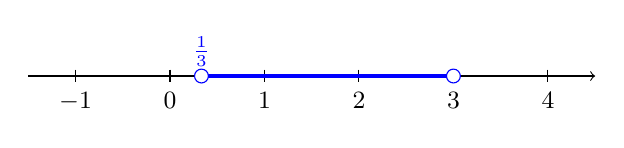
\begin{tikzpicture}[x=1.2cm]
\draw[->] (-1.5,0) -- (4.5,0);
\foreach \t in {-1,0,1,2,3,4} \draw (\t,0.08) -- (\t,-0.08) node[below] {\small $\t$};
\draw[very thick,blue] (1/3,0) -- (3,0);
\draw[blue,fill=white] (1/3,0) circle (2.5pt) node[above] {\small $\frac{1}{3}$};
\draw[blue,fill=white] (3,0) circle (2.5pt);
\end{tikzpicture}
\end{center}
ដូច្នេះ វិសមីការមានចម្លើយ $x \in \left(\dfrac{1}{3}, 3\right)$ ។

គ. វិសមីការមានន័យកាលណា $5x - 3 > 0$ ឬ $x > \dfrac{3}{5}$ ។ ដោយគោល $\frac{1}{2} < 1$ (ប្ដូរទិសដៅវិសមីការ) ៖ $12 > 5x - 3$ នាំឱ្យ $5x < 15$ ឬ $x < 3$ ។
\begin{center}
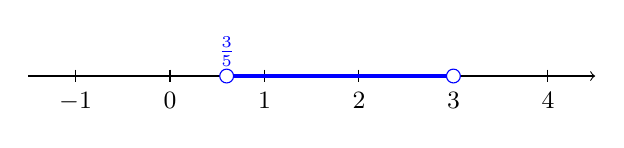
\begin{tikzpicture}[x=1.2cm]
\draw[->] (-1.5,0) -- (4.5,0);
\foreach \t in {-1,0,1,2,3,4} \draw (\t,0.08) -- (\t,-0.08) node[below] {\small $\t$};
\draw[very thick,blue] (0.6,0) -- (3,0);
\draw[blue,fill=white] (0.6,0) circle (2.5pt) node[above] {\small $\frac{3}{5}$};
\draw[blue,fill=white] (3,0) circle (2.5pt);
\end{tikzpicture}
\end{center}
ដូច្នេះ វិសមីការមានចម្លើយ $x \in \left(\dfrac{3}{5}, 3\right)$ ។
\end{example}

\begin{pro}
ដោះស្រាយវិសមីការខាងក្រោម ៖
\begin{tasks}(2)
  \task $\log_2 n > 8$
  \task $\log_{\frac{1}{3}} a < 0$
  \task $\log_8 x \le -2$
  \task $\log(x^2 - 6) > \log x$
\end{tasks}
\ans
ក. $n > 256$ \quad ខ. $a > 1$ \quad គ. $0 < x \le \dfrac{1}{64}$ \quad ឃ. $x > 3$ ។
\end{pro}

\section{លោការីតគោល 10 និងលោការីតនេពែ}
\subsection{លោការីតគោល 10}
\textbf{ឧទាហរណ៍ ៖} គេឱ្យអនុគមន៍ $y = 10^x$ គេបាន $x = \log_{10} y$ ។ កន្សោម $\log_{10} y$ ហៅថា “លោការីតគោល $10$” ។

\textbf{សង្កេត ៖} គេមាន $50 = 10^x$ ។ គេទាញបាន
\[
x = \log_{10} 50 \approx 1.699
\]
ឬ $50 \approx 10^{1.699}$ ។
\begin{center}
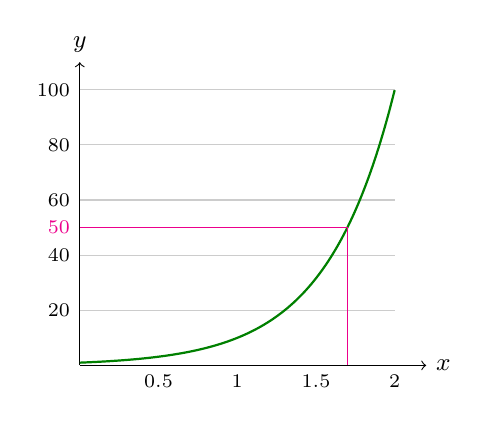
\begin{tikzpicture}[x=2cm,y=0.035cm]
\draw[->] (0,0) -- (2.2,0) node[right] {\small $x$};
\draw[->] (0,0) -- (0,110) node[above] {\small $y$};
\foreach \t in {20,40,60,80,100} {\draw[gray!40] (0,\t) -- (2,\t); \node[left] at (0,\t) {\scriptsize $\t$};}
\foreach \t in {0.5,1,1.5,2} \node[below] at (\t,0) {\scriptsize $\t$};
\draw[thick,green!50!black,domain=0:2,samples=60,smooth] plot (\x,{10^(\x)});
\draw[magenta] (0,50) -- (1.699,50) -- (1.699,0);
\node[left,magenta] at (0,50) {\scriptsize $50$};
\end{tikzpicture}
\end{center}

\begin{definition}[និយមន័យ]
\textbf{លោការីតគោល $10$} នៃអថេរមួយ ជាកន្សោមនៃនិទស្សន្តស្វ័យគុណដែលតម្លៃរបស់វាបានមកដោយយក $10$ ជាគោល ហើយត្រូវបានកំណត់សរសេរដោយ $\log_{10} x$ ឬ $\log x$ ។
\end{definition}

\begin{example}[លំហាត់គំរូ]
គេឱ្យសមីការ ក. $10^{2x - 3} = 7$ \quad ខ. $6^{x + 2} = 21$ ។ ចូររកតម្លៃ $x$ ជាអនុគមន៍នៃលោការីតគោល $10$ ។
\ans
ក. $10^{2x - 3} = 7$ គេបាន $2x - 3 = \log 7$ នាំឱ្យ $2x = \log 7 + 3$ ។ ដូច្នេះ $x = \dfrac{\log 7 + 3}{2}$ ។\\
ខ. $6^{x + 2} = 21$ គេបាន $x + 2 = \log_6 21$ នាំឱ្យ $x = \log_6 21 - 2$ ។ ដូច្នេះ $x = \dfrac{\log 21}{\log 6} - 2$ ។
\end{example}

\begin{pro}
ដោះស្រាយសមីការ ៖ \quad ក. $\log(40 + y^2) = 2.5$ \quad ខ. $\log(y + 18) + \log 5 - \log(2y - 3) = 2$ ។
\ans
ក. $y^2 = 10^{2.5} - 40 \approx 276.23$ ដូច្នេះ $y \approx \pm 16.6$ \quad ខ. $5(y + 18) = 100(2y - 3)$ ដូច្នេះ $y = 2$ ។
\end{pro}

\subsection{លោការីតនេពែ}
\textbf{ឧទាហរណ៍ ៖} គេឱ្យអនុគមន៍ $y = e^x$ ដែល $e$ ជាចំនួនអសនិទាន $e \approx 2.718281828459045\ldots$ នោះគេបាន $x = \log_e y$ ។ កន្សោម $\log_e y$ ហៅថា “លោការីតនេពែ” ។

\begin{definition}[និយមន័យ]
\textbf{លោការីតនេពែ} នៃអថេរមួយ ជាកន្សោមនៃនិទស្សន្តស្វ័យគុណដែលតម្លៃរបស់វាបានមកដោយយក $e$ ជាគោល ហើយត្រូវបានកំណត់សរសេរដោយ $\log_e x$ ឬ $\ln x$ ។
\end{definition}

\begin{example}[លំហាត់គំរូ]
គេឱ្យសមីការ ក. $e^{x - 2} = 12$ \quad ខ. $4e^{2x} + 2 = 18$ ។ ចូររកតម្លៃ $x$ ជាអនុគមន៍នៃលោការីតនេពែ ។
\ans
ក. $e^{x - 2} = 12$ គេបាន $x - 2 = \ln 12$ ។ ដូច្នេះ $x = \ln 12 + 2$ ។\\
ខ. $4e^{2x} + 2 = 18$ គេបាន $4e^{2x} = 16$, $e^{2x} = 4$ នាំឱ្យ $2x = \ln 4$ ។ ដូច្នេះ $x = \dfrac{\ln 4}{2} = \ln 2$ ។
\end{example}

\begin{pro}
ដោះស្រាយសមីការ ៖ \quad ក. $e^{5x + 2} = 23$ \quad ខ. $e^x(2e^x - 1) = 10$ ។
\ans
ក. $x = \dfrac{\ln 23 - 2}{5} \approx 0.227$ \quad ខ. តាង $t = e^x > 0$ ៖ $2t^2 - t - 10 = 0$ នាំឱ្យ $t = \dfrac{5}{2}$ ដូច្នេះ $x = \ln 2.5 \approx 0.916$ ។
\end{pro}

\subsection{ក្រាបនៃអនុគមន៍លោការីតគោល 10 និងលោការីតនេពែ}
\[
\begin{gathered}
y = \log_{10} x \iff 10^y = x \quad (\log_{10} x = \log x)\\
y = \log_e x \iff e^y = x \quad (\log_e x = \ln x)
\end{gathered}
\]
\begin{center}
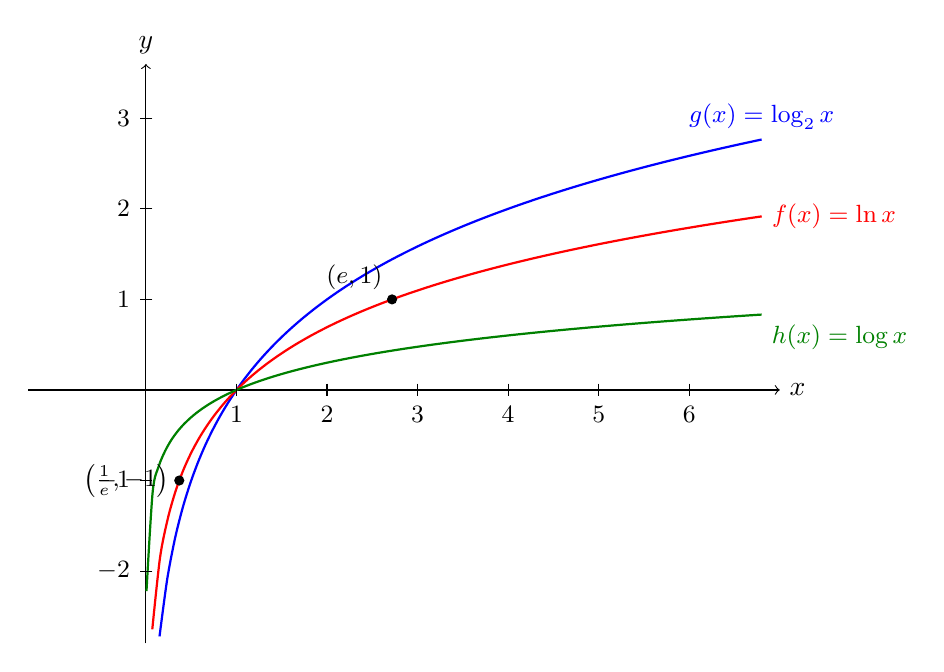
\begin{tikzpicture}[scale=1.15]
\draw[->] (-1.3,0) -- (7,0) node[right] {$x$};
\draw[->] (0,-2.8) -- (0,3.6) node[above] {$y$};
\draw[thick,blue,domain=0.15:6.8,samples=80,smooth] plot (\x,{ln(\x)/ln(2)}) node[above] {\small $g(x) = \log_2 x$};
\draw[thick,red,domain=0.07:6.8,samples=80,smooth] plot (\x,{ln(\x)}) node[right] {\small $f(x) = \ln x$};
\draw[thick,green!50!black,domain=0.006:6.8,samples=100,smooth] plot (\x,{ln(\x)/ln(10)}) node[below right] {\small $h(x) = \log x$};
\fill (2.718,1) circle (1.6pt) node[above left] {\small $(e, 1)$};
\fill (0.368,-1) circle (1.6pt) node[left] {\small $\left(\frac{1}{e}, -1\right)$};
\foreach \t in {1,...,6} \draw (\t,0.07) -- (\t,-0.07) node[below] {\small $\t$};
\foreach \t in {-2,-1,1,2,3} \draw (0.07,\t) -- (-0.07,\t) node[left] {\small $\t$};
\end{tikzpicture}
\end{center}

\begin{formulaBox}[ជាទូទៅ]
តាមក្រាប អនុគមន៍លោការីតដែលមានគោលកាន់តែធំ (ចំពោះគោល $a > 1$) នោះអនុគមន៍មានកំណើនកាន់តែយឺត ។
\end{formulaBox}

\section{ការអនុវត្តលើអនុគមន៍លោការីត}
\subsection{តម្លៃកើនតាមឆ្នាំ}

\begin{example}[ឧទាហរណ៍]
មនុស្សម្នាក់បានយកប្រាក់ចំនួន $2\,925\,000$ រៀល ទៅផ្ញើនៅធនាគារដោយទទួលបានអត្រាការប្រាក់ $10\%$ ក្នុងមួយឆ្នាំ ។ ធនាគារទូទាត់ការប្រាក់មួយឆមាសម្ដង ។ តើរយៈពេលប៉ុន្មានឆ្នាំ ទើបធ្វើឱ្យប្រាក់របស់គាត់កើនដល់ $3\,705\,000$ រៀល?
\ans
តាមរូបមន្ត $A = P\left(1 + \dfrac{r}{n}\right)^{nt}$ ដែល $P = 2\,925\,000$, $r = 0.10$, $n = 2$, $A = 3\,705\,000$ ។ គេបាន
\[
\begin{gathered}
3\,705\,000 = 2\,925\,000\left(1 + \frac{0.10}{2}\right)^{2t} \;\Rightarrow\; \frac{3\,705\,000}{2\,925\,000} = 1.05^{2t}\\
1.2667 = 1.05^{2t} \;\Rightarrow\; \log 1.2667 = 2t\log 1.05\\
t = \frac{\log 1.2667}{2\log 1.05} \approx 2.42
\end{gathered}
\]
ដូច្នេះ ដើម្បីឱ្យប្រាក់របស់គាត់កើនដល់ $3\,705\,000$ រៀល គាត់ត្រូវប្រើពេលអស់ប្រហែល $2.42$ ឆ្នាំ ។
\end{example}

\subsection{តម្លៃថយតាមឆ្នាំ}
\textbf{ឧទាហរណ៍ ៖} បើយើងសង្កេតលើរបស់មួយចំនួនដែលយើងជួបប្រទះរាល់ថ្ងៃ យើងឃើញថាមានរបស់ខ្លះឡើងថ្លៃជារៀងរាល់ថ្ងៃ ដូចជា ដី ផ្ទះ ជាដើម ។ ទន្ទឹមនឹងរបស់ដែលកើនតម្លៃរហូត ក៏មានរបស់ខ្លះចុះថ្លៃរហូតដែរ ដូចជារថយន្ត ម៉ូតូ ជាដើម ។ ឧទាហរណ៍ បើយើងទិញរថយន្តថ្មីមួយគ្រឿងតម្លៃ $20\,000$ ដុល្លារ ហើយតម្លៃរថយន្តនេះនឹងចុះថ្លៃ $15\%$ ជារៀងរាល់ឆ្នាំ នោះតារាងតម្លៃរថយន្តចំនួន $4$ ឆ្នាំក្រោយ បង្ហាញដូចតារាងខាងក្រោម ៖
\[
\begin{array}{|c|c|}\hline
\text{ចំនួនឆ្នាំទិញរថយន្ត} & \text{តម្លៃរថយន្តជាដុល្លារ}\\ \hline
0 & 20\,000\\
1 & 17\,000\\
2 & 14\,450\\
3 & 12\,282.5\\
4 & 10\,440.13\\ \hline
\end{array}
\]
យើងសង្កេតឃើញថា តម្លៃរថយន្តមានការថយចុះជារៀងរាល់ឆ្នាំ ទៅតាមអត្រាភាគរយកំណត់របស់វា ។

\begin{example}[លំហាត់គំរូ]
មនុស្សម្នាក់បានផឹកតែទឹកកកក្រូចឆ្មារមួយកែវ ដែលមានសារជាតិស្ករចំណុះ $130$ មីលីក្រាម ។ បើស្កររលាយចូលក្នុងសរពាង្គកាយក្នុងអត្រា $11\%$ ក្នុងមួយម៉ោង ។ តើរយៈពេលប៉ុន្មានម៉ោង ទើបសារជាតិស្កររលាយចូលក្នុងរាងកាយអស់ពាក់កណ្ដាលនៃបរិមាណស្ករដែលមាន?
\ans
ប្រើរូបមន្ត $y = a(1 - r)^t$ ដោយ $y = \dfrac{130}{2} = 65$, $r = 0.11$, $a = 130$ ។ គេបាន
\[
\begin{gathered}
65 = 130(1 - 0.11)^t \;\Rightarrow\; 0.89^t = 0.5\\
t\log 0.89 = \log 0.5 \;\Rightarrow\; t = \frac{\log 0.5}{\log 0.89} \approx 5.9480
\end{gathered}
\]
ដូច្នេះ ដើម្បីឱ្យស្ករជ្រាបចូលក្នុងរាងកាយអស់ពាក់កណ្ដាល គេត្រូវប្រើពេលប្រហែល $6$ ម៉ោង ។
\end{example}

\begin{pro}
\begin{enumerate}[a]
  \item ពូសៅបានយកប្រាក់ចំនួន $2\,000\,000$ រៀល ទៅផ្ញើនៅធនាគារដោយទទួលបានអត្រាការប្រាក់ $6\%$ ក្នុងមួយឆ្នាំ ។ តើរយៈពេលប៉ុន្មានឆ្នាំ ទើបប្រាក់របស់គាត់កើនឡើងពីរដង?
  \item គ្រឹះស្ថានបោះពុម្ពនិងចែកផ្សាយបានទិញកុំព្យូទ័រមួយគ្រឿងថ្លៃ $3\,000$ ដុល្លារ ។ បើគេគិតប្រាក់រំលស់ $20\%$ ជារៀងរាល់ឆ្នាំ ចូររកតម្លៃកុំព្យូទ័រក្នុងរយៈពេល $3$ ឆ្នាំក្រោយ ។
  \item តាមការស្រង់ស្ថិតិឆ្នាំ $2000$ ប្រទេសចិនមានប្រជាជន $1.26$ ពាន់លាននាក់ ដែលជាចំនួនច្រើនជាងគេបំផុតនៅលើពិភពលោក ។ ប្រទេសដែលមានចំនួនប្រជាជនច្រើនបន្ទាប់ពីប្រទេសចិន គឺប្រទេសឥណ្ឌា ដែលមានចំនួន $1.01$ ពាន់លាននាក់ ។ ចំនួនប្រជាជននៃប្រទេសឥណ្ឌានិងប្រទេសចិន អាចគណនាតាមសមីការ $I(t) = 1.01e^{0.015t}$ និង $C(t) = 1.26e^{0.009t}$ (គេកំណត់ $e \approx 2.7183$) ។ តាមសមីការគំរូទាំងពីរ តើនៅឆ្នាំណាដែលប្រទេសឥណ្ឌាកើនចំនួនប្រជាជនច្រើនជាងប្រទេសចិន?
\end{enumerate}
\ans
ក. $1.06^t = 2$ នាំឱ្យ $t = \dfrac{\log 2}{\log 1.06} \approx 11.9$ ឆ្នាំ (ប្រហែល $12$ ឆ្នាំ) ។\\
ខ. $3\,000(1 - 0.2)^3 = \$1\,536$ ។\\
គ. $1.01e^{0.015t} > 1.26e^{0.009t}$ នាំឱ្យ $e^{0.006t} > \dfrac{1.26}{1.01}$ ឬ $t > \dfrac{1}{0.006}\ln\dfrac{1.26}{1.01} \approx 36.9$ ។ ដូច្នេះ នៅឆ្នាំ $2037$ ។
\end{pro}

\section*{មេរៀនសង្ខេប ជំពូកទី ២}
\begin{note}[មេរៀនសង្ខេប]
\textbf{១. អនុគមន៍អិចស្ប៉ូណង់ស្យែល}
\begin{itemize}
  \item ស្វ័យគុណ ៖ $\underbrace{a\cdot a\cdots a}_{n \text{ កត្តា}} = a^n$ ដែល $n \in \mathbb{N}$ ។ បើ $a$, $b$ ជាចំនួនពិត ហើយ $m$, $n$ ជាចំនួនគត់វិជ្ជមាន គេបាន ៖
  \[
  \begin{gathered}
  a^m\times a^n = a^{m+n},\quad (a^m)^n = a^{mn}\\
  (ab)^n = a^nb^n,\quad \left(\frac{a}{b}\right)^n = \frac{a^n}{b^n}\ (b \ne 0)\\
  \frac{a^m}{a^n} = a^{m-n},\quad a^0 = 1,\quad \frac{1}{a^n} = a^{-n}\ (a \ne 0)
  \end{gathered}
  \]
  \item ឫសទី $n$ ៖ បើ $a$ ជាចំនួនពិត $\sqrt[n]{a^n} = |a|$ បើ $n$ ជាចំនួនគត់គូ និង $\sqrt[n]{a^n} = a$ បើ $n$ ជាចំនួនគត់សេស ។
  \[
  \begin{gathered}
  \sqrt[n]{a}\cdot\sqrt[n]{b} = \sqrt[n]{ab},\quad \sqrt[n]{\frac{a}{b}} = \frac{\sqrt[n]{a}}{\sqrt[n]{b}}\ (b \ne 0),\quad \sqrt[n]{a^m} = a^{\frac{m}{n}}\\
  \sqrt[n]{\sqrt[k]{a}} = \sqrt[nk]{a},\quad \sqrt[nk]{a^{mk}} = \sqrt[n]{a^m}
  \end{gathered}
  \]
  \item បើ $a > 0$, $a \ne 1$ នោះ $a^x = a^y$ សមមូល $x = y$ ។
  \item អនុគមន៍អិចស្ប៉ូណង់ស្យែលកំណត់ដោយ $f(x) = a^x$, $x \in \mathbb{R}$, $a > 0$ និង $a \ne 1$ ។
  \item បើ $P$ ប្រាក់ដើម $i$ អត្រាការប្រាក់ប្រចាំឆ្នាំ $n$ ជាចំនួនឆ្នាំ ប្រាក់សរុបគឺ $A = P(1 + i)^n$ ។
\end{itemize}
\textbf{២. អនុគមន៍លោការីត}
\begin{itemize}
  \item បើ $(a, b)$ ផ្ទៀងផ្ទាត់ $f(x)$ ហើយ $(b, a)$ ផ្ទៀងផ្ទាត់ $f^{-1}(x)$ នោះ $f^{-1}(x)$ ជាអនុគមន៍ច្រាសនៃអនុគមន៍ $f(x)$ ។
  \item បើអនុគមន៍ពីរច្រាសគ្នា នោះក្រាបនៃអនុគមន៍ទាំងពីរឆ្លុះគ្នាធៀបនឹងបន្ទាត់ $y = x$ ។
  \item បើ $a^x = y$ នោះ $x = \log_a y$, $y > 0$, $a > 0$, $a \ne 1$ ហើយ $f(x) = a^x$ មានអនុគមន៍ច្រាស $f^{-1}(x) = \log_a x$ ។
  \item លក្ខណៈលោការីត ៖ ចំពោះគ្រប់ $x > 0$, $y > 0$, $a > 0$, $a \ne 1$ និង $b > 0$, $b \ne 1$ ៖
  \[
  \begin{gathered}
  \log_a(xy) = \log_a x + \log_a y,\quad \log_a x^n = n\log_a x\\
  \log_a\left(\frac{x}{y}\right) = \log_a x - \log_a y\\
  \log_a b = \frac{1}{\log_b a},\quad \log_a x = \frac{\log_b x}{\log_b a}\\
  \log_a a = 1,\quad \log_a 1 = 0\\
  \log_a a^x = x,\quad a^{\log_a x} = x
  \end{gathered}
  \]
\end{itemize}
\end{note}

\section*{លំហាត់ជំពូកទី ២}
\begin{enumerate}[1]
  \item ដោះស្រាយសមីការអិចស្ប៉ូណង់ស្យែល ៖
  \begin{tasks}(2)
    \task $3^{x^2} = 81^{x - 1}$
    \task $9^{(2x - 1)^2} = 3^{x + 3}$
    \task $2(3)^{2x + 3} = 3 - 7(3^x)$
    \task $2^{2x + 3} - 2^x = 1 - 2^{x + 3}$
  \end{tasks}
  \item បើ $a^x = b^y = (ab)^z$ ។ បង្ហាញថា $xy = z(x + y)$ ។
  \item បើ $2^x = 3^y = 12^z$ ។ បង្ហាញថា $xy = z(x + 2y)$ ។
  \item បើ $a = \sqrt{3} + \sqrt{2}$ និង $b = \sqrt{3} - \sqrt{2}$ ។ បង្ហាញថា $\dfrac{1}{1 + a} + \dfrac{1}{1 + b} = 1$ ។
  \item បើ $a^2 + b^2 = 11ab$ ។ បង្ហាញថា $\log a + \log b = 2\log\left(\dfrac{a - b}{3}\right)$ ។
  \item បើ $\log_x M = a$ និង $\log_y M = b$ ។ បង្ហាញថា $\log_{xy} M = \dfrac{ab}{a + b}$ ។
  \item ដោះស្រាយសមីការលោការីត ៖
  \begin{tasks}(2)
    \task $2 + \log_{10}(2x - 3) = \log_{10} x^2 + \log_{10} 25$
    \task $6(\log_x 8 + \log_8 x) = 13$
    \task $\log_x 9 + \log_9 x = \dfrac{5}{2}$
    \task $\log_9 x + \log_{x^2} 9 = 1$
  \end{tasks}
  \item ដោះស្រាយវិសមីការអិចស្ប៉ូណង់ស្យែល ៖
  \begin{tasks}(2)
    \task $25^x \ge 125^{3x - 2}$
    \task $3^x > 27$
    \task $4^x - 6(2^x) + 8 > 0$
    \task $15^x \ge \dfrac{1}{\sqrt[4]{15^3}}$
    \task $\left(\dfrac{1}{5}\right)^x < \sqrt[3]{0.04}$
    \task $(0.3)^x \le \dfrac{100}{9}$
  \end{tasks}
  \item ដោះស្រាយវិសមីការលោការីត ៖
  \begin{tasks}(2)
    \task $\log_{3x - 2} x \le 1$
    \task $\log_2^2 x - \log_2 x - 15 < 0$
    \task $\log_4(3^x - 1)\cdot\log_{\frac{1}{4}}\dfrac{3^x - 1}{16} = \dfrac{3}{4}$
    \task $x\cdot\log_{0.1}(x^2 + x + 1) \ge 0$
    \task $\log_{\frac{x}{5}}(x^2 - 8x + 16) \le 0$
    \task $\log_{x - \frac{9}{2}}\dfrac{x + 4}{2x - 6} \le \log_{x - \frac{9}{2}}(x - 5)$
  \end{tasks}
  \item មនុស្សម្នាក់បានយកប្រាក់ទៅផ្ញើនៅធនាគារអេស៊ីលីដាចំនួន $1\,000\$$ ដោយទទួលបានអត្រាការប្រាក់ $4\%$ ក្នុងមួយឆ្នាំ ។ បើគាត់វិនិយោគប្រាក់នេះតាំងពីឆ្នាំ $1996$ មក តើបច្ចុប្បន្ននេះឆ្នាំ $2007$ គាត់មានប្រាក់សរុបទាំងអស់ប៉ុន្មាននៅធនាគារ?
  \item គេឱ្យអនុគមន៍ $f(x) = a^x$ និងអនុគមន៍ច្រាស $f^{-1}(x) = \log_a x$ ដែល $a$ ជាចំនួនពិតវិជ្ជមាននិង $a \ne 1$ ។
  \begin{enumerate}[a]
    \item រកតម្លៃ $a$ ដើម្បីឱ្យក្រាបនៃអនុគមន៍ $f(x)$ និង $f^{-1}(x)$ កាត់គ្នា ។
    \item រកគ្រប់ចំណុចដែលក្រាបនៃអនុគមន៍ទាំងពីរកាត់គ្នា (ក្នុងសំណួរ ក) ។
  \end{enumerate}
\end{enumerate}

\section*{លំហាត់អនុវត្តន៍}
\begin{enumerate}[1]
  \item រកសមីការនៃអនុគមន៍ច្រាសរបស់អនុគមន៍ខាងក្រោម ៖
  \begin{tasks}(4)
    \task $y = 4x - 3$
    \task $y = 3x^2 + 1$
    \task $x^2 - 3y^2 = 3$
    \task $xy = -6$
    \task $xy^2 = 1$
    \task $\dfrac{x^2}{9} + \dfrac{y^2}{4} = 1$
    \task $y = \dfrac{5}{x}$
    \task $y = \sqrt{x - 2}$
  \end{tasks}
  \ans
  ក. $y = \dfrac{x + 3}{4}$ \quad ខ. $y = \pm\sqrt{\dfrac{x - 1}{3}}$ ($x \ge 1$) \quad គ. $y^2 - 3x^2 = 3$ ឬ $y = \pm\sqrt{3x^2 + 3}$ \quad ឃ. $y = -\dfrac{6}{x}$ \quad ង. $x^2y = 1$ ឬ $y = \dfrac{1}{x^2}$ \quad ច. $\dfrac{x^2}{4} + \dfrac{y^2}{9} = 1$ \quad ឆ. $y = \dfrac{5}{x}$ \quad ជ. $y = x^2 + 2$ ($x \ge 0$) ។
  \item គេឱ្យអនុគមន៍ $f(x) = x - 2$ ។ ចូរកំណត់អនុគមន៍ច្រាស $f^{-1}(x)$ រួចសង់ក្រាបរបស់វា ។
  \ans
  $f^{-1}(x) = x + 2$ ។ ក្រាបទាំងពីរជាបន្ទាត់ស្របគ្នា ឆ្លុះគ្នាធៀបនឹងបន្ទាត់ $y = x$ ។
  \item សង់ក្រាបនៃអនុគមន៍ខាងក្រោម ៖
  \begin{tasks}(3)
    \task $y = \log_5 x$
    \task $y = \log_7 x$
    \task $y = \log_{10} x$
    \task $y = \log_{1.5} x$
    \task $y = \log_{0.5} x$
    \task $y = \log_{0.3} x$
  \end{tasks}
  \ans
  ក្រាបទាំងអស់កាត់តាម $(1, 0)$ និង $(a, 1)$ ។ ក, ខ, គ, ឃ ជាអនុគមន៍កើន (គោល $a > 1$) ហើយ ង, ច ជាអនុគមន៍ចុះ (គោល $0 < a < 1$) ។
  \item បំប្លែងជាទម្រង់លោការីត ៖
  \begin{tasks}(4)
    \task $10^4 = 10000$
    \task $8^{\frac{1}{3}} = 2$
    \task $16^{\frac{1}{4}} = 2$
    \task $5^{-2} = \frac{1}{25}$
    \task $4^{-3} = \frac{1}{64}$
    \task $10^{0.3010} = 2$
    \task $x^{-a} = y$
    \task $A = k^c$
  \end{tasks}
  \ans
  ក. $\log 10000 = 4$ \quad ខ. $\log_8 2 = \frac{1}{3}$ \quad គ. $\log_{16} 2 = \frac{1}{4}$ \quad ឃ. $\log_5\frac{1}{25} = -2$ \quad ង. $\log_4\frac{1}{64} = -3$ \quad ច. $\log 2 = 0.3010$ \quad ឆ. $\log_x y = -a$ \quad ជ. $\log_k A = c$ ។
  \item សម្រួល ៖
  \begin{tasks}(4)
    \task $3^{\log_3 2}$
    \task $5^{\log_5 10}$
    \task $\log_a a^{10}$
    \task $\log_q q^a$
    \task $\log_4 64$
    \task $\log_{10} 0.1$
    \task $\log_{\sqrt{2}} 16$
    \task $\log_{10} 1$
  \end{tasks}
  \ans
  ក. $2$ \quad ខ. $10$ \quad គ. $10$ \quad ឃ. $a$ \quad ង. $3$ \quad ច. $-1$ \quad ឆ. $8$ \quad ជ. $0$ ។
  \item ដោះស្រាយសមីការលោការីត ៖
  \begin{tasks}(3)
    \task $\log_3 x = 3$
    \task $\log_x 16 = 2$
    \task $\log x + \log(x + 9) = 1$
    \task $\log_2 x = -1$
    \task $\log_9 x = \frac{1}{2}$
    \task $\log_8 x = \frac{1}{3}$
    \task $\log\sqrt[3]{x} = \sqrt{\log x}$
    \task $\log_5\sqrt{x^2 + 1} = \sqrt{1}$
    \task $\log_4(x + 3) + \log_4(x - 3) = 2$
    \task $\log\sqrt[3]{x^2} + \log\sqrt[3]{x^4} = \log 2^{-3}$
  \end{tasks}
  \ans
  ក. $x = 27$ \quad ខ. $x = 4$ \quad គ. $x(x + 9) = 10$ ដូច្នេះ $x = 1$ \quad ឃ. $x = \frac{1}{2}$ \quad ង. $x = 3$ \quad ច. $x = 2$ \quad ឆ. តាង $t = \log x \ge 0$ ៖ $\frac{t}{3} = \sqrt{t}$ នាំឱ្យ $t = 0$ ឬ $t = 9$ ដូច្នេះ $x = 1$ ឬ $x = 10^9$ \quad ជ. $\sqrt{x^2 + 1} = 5$ ដូច្នេះ $x = \pm 2\sqrt{6}$ \quad ឈ. $x^2 - 9 = 16$ ដូច្នេះ $x = 5$ \quad ញ. $2\log|x| = -3\log 2$ ដូច្នេះ $x = \pm\dfrac{\sqrt{2}}{4}$ ។
  \item ដោះស្រាយវិសមីការលោការីត ៖
  \begin{tasks}(3)
    \task $\log_2 2x \le \log_4(x + 3)$
    \task $\log_3(3x - 5) \ge \log_3(x + 7)$
    \task $\log\dfrac{x^2 - x}{x^2 - 1} < 0$
    \task $\log_{0.5} x^2 < \log_{0.5} 3x$
    \task $\log_5 12 < \log_5(5x - 3)$
    \task $\log(x^2 - 2x + 3) \ge 0$
    \task $\log_8(3x - 1) < \log_8(x + 5)$
  \end{tasks}
  \ans
  ក. $\log_4 4x^2 \le \log_4(x + 3)$ នាំឱ្យ $4x^2 - x - 3 \le 0$ ដូច្នេះ $0 < x \le 1$ \quad ខ. $x \ge 6$ \quad គ. $0 < \dfrac{x}{x + 1} < 1$ ($x \ne 1$) ដូច្នេះ $x \in (0, 1) \cup (1, +\infty)$ \quad ឃ. $x^2 > 3x$, $x > 0$ ដូច្នេះ $x > 3$ \quad ង. $x > 3$ \quad ច. $(x - 1)^2 + 2 \ge 1$ ពិតជានិច្ច ដូច្នេះ $x \in \mathbb{R}$ \quad ឆ. $x \in \left(\dfrac{1}{3}, 3\right)$ ។
  \item ពូសេងយកប្រាក់ $4\,000\,000$ រៀល ទៅធ្វើវិនិយោគទុន ដោយទទួលបានអត្រាការប្រាក់ $6\%$ ក្នុងមួយឆ្នាំ ។ តើប៉ុន្មានឆ្នាំក្រោយ ទើបប្រាក់របស់គាត់កើនឡើងពីរដង?
  \ans
  $1.06^t = 2$ នាំឱ្យ $t = \dfrac{\log 2}{\log 1.06} \approx 11.9$ ឆ្នាំ (ប្រហែល $12$ ឆ្នាំ) ។
  \item មីងសុខាបានទិញរថយន្តថ្មីមួយគ្រឿងថ្លៃ $38\,500$ ដុល្លារ ។ បើរថយន្តចុះថ្លៃក្នុងអត្រា $15\%$ ក្នុងមួយឆ្នាំ ។ តើរយៈពេល $7$ ឆ្នាំក្រោយ រថយន្តគាត់នៅសល់ថ្លៃប៉ុន្មាន?
  \ans
  $38\,500(0.85)^7 \approx \$12\,342.22$ ។
\end{enumerate}
